\section{Bilinear weight interpolation}
\label{app:bilinear}

Continuous-in-depth work treats the weights as a function of depth $\theta(t)$ expanded
in a basis~\citep{queiruga2020continuousindepthneuralnetworks}.
The piecewise-constant basis recovers a ResNet, and multi-level training refines depth
by copying adjacent blocks~\citep{chang2018multilevel}; smoother bases are a natural
alternative.
We test the simplest one, linear interpolation between consecutive blocks,
\begin{equation}
    \theta(t) \;=\; (1-\alpha)\,\theta_i + \alpha\,\theta_{i+1},
    \qquad \alpha = t - i.
    \label{eq:bilinear-theta}
\end{equation}
Replacing the piecewise-constant schedule $\theta_t=\theta_{\lfloor t\rfloor}$ by~\eqref{eq:bilinear-theta}
hurts every model we tested: at $R{=}128$ the drop against the piecewise-constant schedule is between $6.6$ and $23.3$
points (\cref{tab:app-bilinear}).
Nothing aligns the hidden units of consecutive blocks; as for independently trained
networks, averaging weights that are not permutation-aligned need not give a functional
intermediate~\citep{entezari2022permutation,ainsworth2023gitrebasin}.

\begin{table}[t]
    \centering
    \caption{Bilinear weight interpolation, Euler, top-1 (\%).}
    \label{tab:app-bilinear}
    \small
    \setlength{\tabcolsep}{2.8pt}
    \begin{tabular}{lrrrrr}
        \toprule
        $R$ & CNX-T & CNX-T$^{\dagger}$ & Swin-T & R-50 & R-101 \\
        \midrule
        1   & 80.96 & 79.27 & 81.08 & 80.34 & 81.67 \\
        2   & 78.94 & 72.43 & 78.93 & 74.95 & 72.55 \\
        4   & 76.16 & 63.13 & 75.42 & 70.60 & 62.42 \\
        10  & 74.42 & 58.75 & 73.28 & 68.58 & 58.73 \\
        128 & 73.66 & 57.44 & 72.14 & 67.77 & 57.73 \\
        \midrule
        $\Delta$ at $R{=}128$ & $-6.6$ & $-19.6$ & $-8.2$ & $-11.7$ & $-23.3$ \\
        \bottomrule
    \end{tabular}
    \vspace{2pt}
    {\footnotesize $^{\dagger}$ConvNeXt-T trained without drop path.}
\end{table}

\Cref{fig:bilinear-norm} shows the ConvNeXt residual-field norm under the piecewise-constant and bilinear
schedules at $R{=}100$.
The piecewise-constant schedule keeps the staircase of \cref{fig:refinement}~(right);
bilinear adds high-frequency oscillation between block boundaries while preserving the
same global growth of $\|f\|$.
Bands are P5--P95 across 500 validation images (same suite as \cref{fig:refinement}).

\begin{figure}[t]
    \centering
    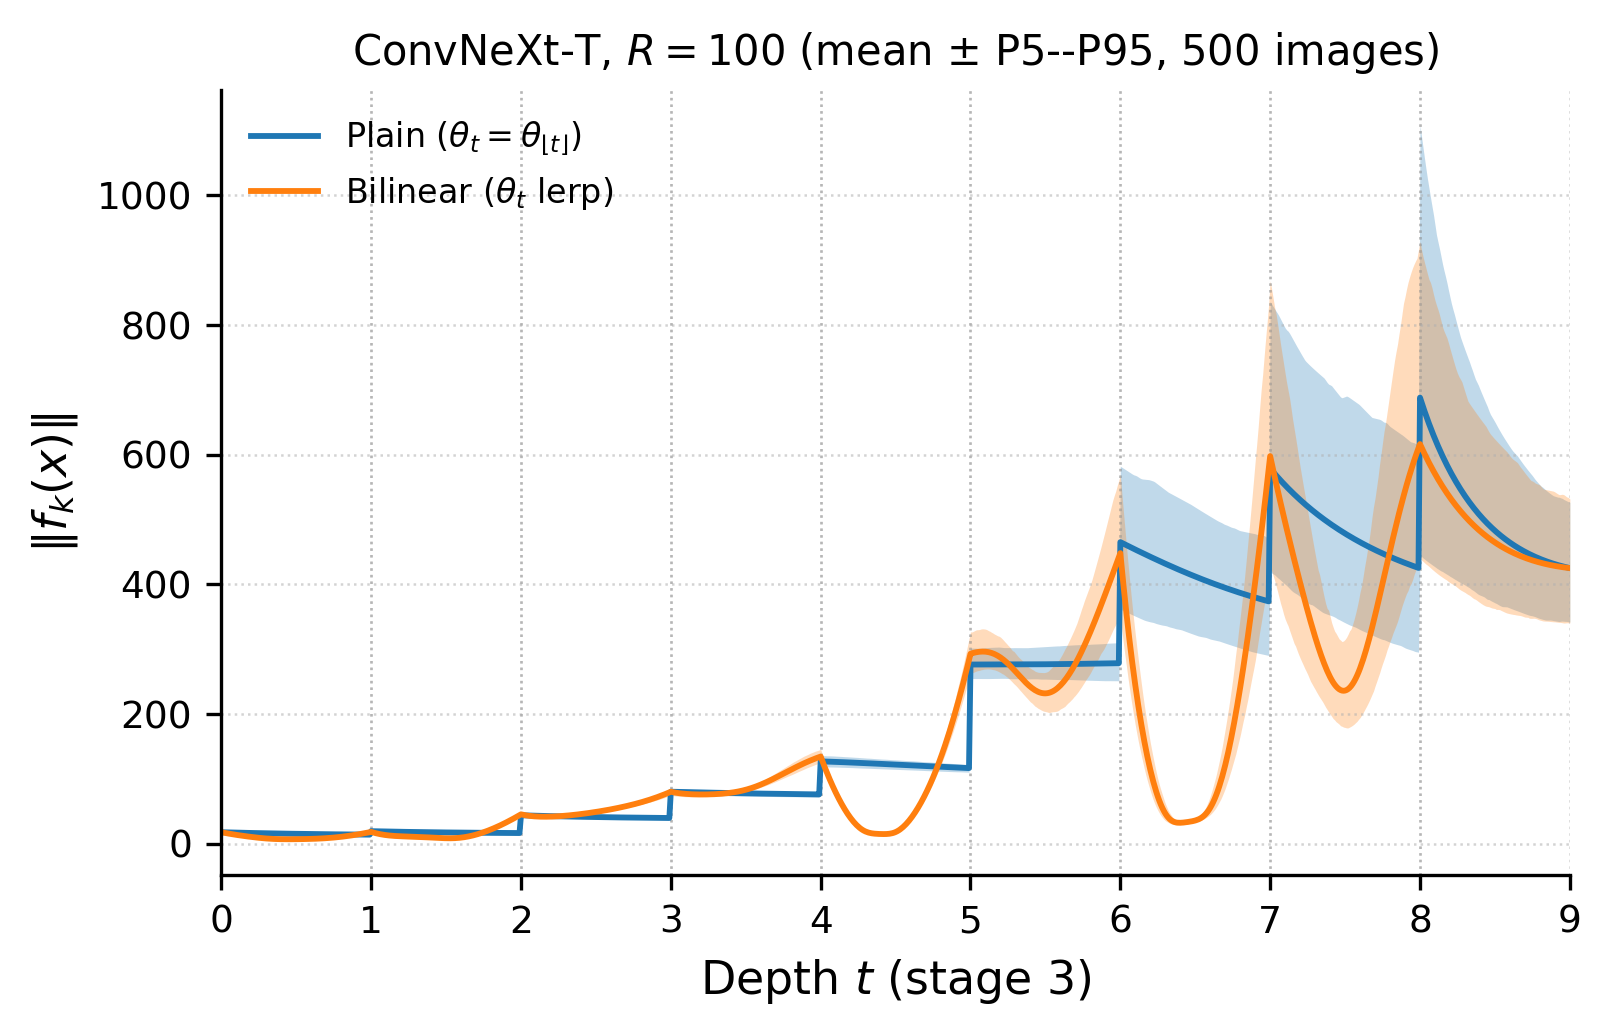
\includegraphics[width=\linewidth]{figures/bilinear_norm.png}
    \caption{ConvNeXt-T residual norm along stage~3 at $R{=}100$:
    piecewise-constant against bilinear weights (mean and P5--P95 over 500 images).}
    \label{fig:bilinear-norm}
\end{figure}
